
\documentclass[a4paper,11pt]{article}
\usepackage[a4paper, margin=8em]{geometry}

% usa i pacchetti per la scrittura in italiano
\usepackage[french,italian]{babel}
\usepackage[T1]{fontenc}
\usepackage[utf8]{inputenc}
\frenchspacing 

% usa i pacchetti per la formattazione matematica
\usepackage{amsmath, amssymb, amsthm, amsfonts}

% usa altri pacchetti
\usepackage{gensymb}
\usepackage{hyperref}
\usepackage{standalone}

% imposta il titolo
\title{Appunti Elettronica Digitale}
\author{Luca Seggiani}
\date{2026}

% imposta lo stile
% usa helvetica
\usepackage[scaled]{helvet}
% usa palatino
\usepackage{palatino}
% usa un font monospazio guardabile
\usepackage{lmodern}

\renewcommand{\rmdefault}{ppl}
\renewcommand{\sfdefault}{phv}
\renewcommand{\ttdefault}{lmtt}

% disponi il titolo
\makeatletter
\renewcommand{\maketitle} {
	\begin{center} 
		\begin{minipage}[t]{.8\textwidth}
			\textsf{\huge\bfseries \@title} 
		\end{minipage}%
		\begin{minipage}[t]{.2\textwidth}
			\raggedleft \vspace{-1.65em}
			\textsf{\small \@author} \vfill
			\textsf{\small \@date}
		\end{minipage}
		\par
	\end{center}

	\thispagestyle{empty}
	\pagestyle{fancy}
}
\makeatother

% disponi teoremi
\usepackage{tcolorbox}
\newtcolorbox[auto counter, number within=section]{theorem}[2][]{%
	colback=blue!10, 
	colframe=blue!40!black, 
	sharp corners=northwest,
	fonttitle=\sffamily\bfseries, 
	title=~\thetcbcounter: #2, 
	#1
}

% disponi definizioni
\newtcolorbox[auto counter, number within=section]{definition}[2][]{%
	colback=red!10,
	colframe=red!40!black,
	sharp corners=northwest,
	fonttitle=\sffamily\bfseries,
	title=~\thetcbcounter: #2,
	#1
}

% U.D.M
\newcommand{\amp}{\ensuremath{\mathrm{A}}}
\newcommand{\volt}{\ensuremath{\mathrm{V}}}
\newcommand{\meter}{\ensuremath{\mathrm{m}}}
\newcommand{\second}{\ensuremath{\mathrm{s}}}
\newcommand{\farad}{\ensuremath{\mathrm{F}}}
\newcommand{\henry}{\ensuremath{\mathrm{H}}}
\newcommand{\siemens}{\ensuremath{\mathrm{S}}}

% circuiti
\usepackage{circuitikz}
\usetikzlibrary{babel}

% disegni
\usepackage{pgfplots}
\pgfplotsset{width=10cm,compat=1.9}

% disponi codice
\usepackage{listings}
\usepackage[table]{xcolor}

\definecolor{codegreen}{rgb}{0,0.6,0}
\definecolor{codegray}{rgb}{0.5,0.5,0.5}
\definecolor{codepurple}{rgb}{0.58,0,0.82}
\definecolor{backcolour}{rgb}{0.95,0.95,0.92}

\lstdefinestyle{codestyle}{
		backgroundcolor=\color{black!5}, 
		commentstyle=\color{codegreen},
		keywordstyle=\bfseries\color{magenta},
		numberstyle=\sffamily\tiny\color{black!60},
		stringstyle=\color{green!50!black},
		basicstyle=\ttfamily\footnotesize,
		breakatwhitespace=false,         
		breaklines=true,                 
		captionpos=b,                    
		keepspaces=true,                 
		numbers=left,                    
		numbersep=5pt,                  
		showspaces=false,                
		showstringspaces=false,
		showtabs=false,                  
		tabsize=2
}

\lstdefinestyle{shellstyle}{
		backgroundcolor=\color{black!5}, 
		basicstyle=\ttfamily\footnotesize\color{black}, 
		commentstyle=\color{black}, 
		keywordstyle=\color{black},
		numberstyle=\color{black!5},
		stringstyle=\color{black}, 
		showspaces=false,
		showstringspaces=false, 
		showtabs=false, 
		tabsize=2, 
		numbers=none, 
		breaklines=true
}

\lstdefinelanguage{javascript}{
	keywords={typeof, new, true, false, catch, function, return, null, catch, switch, var, if, in, while, do, else, case, break},
	keywordstyle=\color{blue}\bfseries,
	ndkeywords={class, export, boolean, throw, implements, import, this},
	ndkeywordstyle=\color{darkgray}\bfseries,
	identifierstyle=\color{black},
	sensitive=false,
	comment=[l]{//},
	morecomment=[s]{/*}{*/},
	commentstyle=\color{purple}\ttfamily,
	stringstyle=\color{red}\ttfamily,
	morestring=[b]',
	morestring=[b]"
}

% disponi sezioni
\usepackage{titlesec}

\titleformat{\section}
	{\sffamily\Large\bfseries} 
	{\thesection}{1em}{} 
\titleformat{\subsection}
	{\sffamily\large\bfseries}   
	{\thesubsection}{1em}{} 
\titleformat{\subsubsection}
	{\sffamily\normalsize\bfseries} 
	{\thesubsubsection}{1em}{}

% disponi alberi
\usepackage{forest}

\forestset{
	rectstyle/.style={
		for tree={rectangle,draw,font=\large\sffamily}
	},
	roundstyle/.style={
		for tree={circle,draw,font=\large}
	}
}

% disponi algoritmi
\usepackage{algorithm}
\usepackage{algorithmic}
\makeatletter
\renewcommand{\ALG@name}{Algoritmo}
\makeatother

% disponi numeri di pagina
\usepackage{fancyhdr}
\fancyhf{} 
\fancyfoot[L]{\sffamily{\thepage}}

\makeatletter
\fancyhead[L]{\raisebox{1ex}[0pt][0pt]{\sffamily{\@title \ \@date}}} 
\fancyhead[R]{\raisebox{1ex}[0pt][0pt]{\sffamily{\@author}}}
\makeatother

\begin{document}
% sezione (data)
\section{Lezione del 24-04-26}

% stili pagina
\thispagestyle{empty}
\pagestyle{fancy}

% testo
\subsection{Amplificatori differenziali}
Iniziamo a vedere gli \textbf{amplificatori differenziali}, di cui un caso particolare sarà l'\textit{amplificatore operazionale} che vedremo in seguito.

Un amplificatore differenziale è un amplificatore che amplifica la differenza fra 2 segnali. Come caso particolare, avremo che amplifica \textit{esclusivamente} la differenza fra 2 segnali.

\begin{center}
\begin{tikzpicture}[transform shape]
	% Paths, nodes and wires:
	\node[op amp, yscale=-1] at (0, -0){};
	\node[shape=rectangle, minimum width=0.465cm, minimum height=0.465cm] at (-1.44, 0.49){} node[anchor=center, align=center, text width=0.077cm, inner sep=6pt] at (-1.6, 0.49){$v_1$};
	\node[shape=rectangle, minimum width=0.465cm, minimum height=0.465cm] at (-1.44, -0.49){} node[anchor=center, align=center, text width=0.077cm, inner sep=6pt] at (-1.6, -0.49){$v_2$};
	\node[shape=rectangle, minimum width=0.465cm, minimum height=0.465cm] at (1.44, -0){} node[anchor=center, align=center, text width=0.077cm, inner sep=6pt] at (1.44, -0){$v_u$};
	\node[ground] at (-0.083, -0.539){};
\end{tikzpicture}
\end{center}

Possiamo vederlo come un componente astratto dotato di due terminali, $v_1$ e $v_2$, da un uscita $v_u$ e da un nodo di riferimento a ground. L'idea fondamentale è che l'uscita $v_u$ abbia valore determinato da:
$$
v_u = K(v_1 - v_2)
$$

\subsubsection{Modo differenziale e modo comune}
Abbiamo infatti due tipologie di segnale:
$$
v_d = (v_1 - v_2) \ \text{modo differenziale}, \quad v_c = \frac{v_1 + v_2}{2} \ \text{modo comune}
$$
che attraverseranno il nostro amplificatore, cioè un segnale a \textit{modo differenziale} dato dalla differenza fra i segnali in entrata, e un segnale a \textit{modo comune} dato dalla loro media. Definiamo quindi 2 guadagni:
$$
A_d = \frac{v_u}{v_d} \ \text{guadagno differenziale}, \quad A_c = \frac{v_u}{v_c} \ \text{guadagno comune}
$$
per i segnali differenziali e comune dell'amplificatore. Ciò che vogliamo in un amplificatore differenziale sarà a questo punto soddisfare:
$$
A_d = K, \quad A_c = 0
$$
Questo non può essere mai fatto in maniera ideale ($A_c$ non sarà mai nullo), per cui si introduce un ulteriore parametro detto \textbf{CMRR} (\textit{Common Mode Rejection Ratio}) definito come:
$$
\text{CMRR} = \frac{A_d}{A_c} \, \mathrm{dB}
$$
In genere si vuole un CMRR che tende ad infinito, mentre nella pratica sta intorno agli $80-150 \, \mathrm{dB}$.

\par\smallskip

\noindent
\textbf{\textsf{Interpretazione geometrica}} \\
\noindent
Possiamo dare un'intepretazione geometrica del rapporto fra $A_d$ e $A_c$ sottraendo le equazioni per il modo differenziale e il modo comune:
$$
\begin{cases}
	v_d = (v_1 - v_2) \\
	v_c = \frac{v_1 + v_2}{2}
\end{cases}
\implies
\begin{cases}
	\frac{v_d}{2} - v_c = \frac{v_1}{2} - \frac{v_2}{2} + \frac{v_1}{2} + \frac{v_2}{2} = v_1 \\
	\frac{v_d}{2} - v_c = \frac{v_1}{2} + \frac{v_2}{2} - \frac{v_1}{2} + \frac{v_2}{2} = v_2 \\
\end{cases}
$$
Si ottengono quindi le espressioni alternative per $v_1$ e $v_2$ in termini del modo differenziale e comune:
$$
v_1 = v_c + \frac{v_d}{2}, \quad  
v_2 = v_c - \frac{v_d}{2} 
$$

Potremmo voler fare la stessa cosa anche per i guadagni, cioè dire:
$$
v_u = v_1 A_1 + v_2 A_2 
= \left( v_c + \frac{v_d}{2} \right) A_1 + \left( v_c - \frac{v_d}{2} \right) A_2 
= v_c (A_1 + A_2) + v_d \left( \frac{A_1 - A_2}{2} \right) = v_c A_c + v_d A_d
$$
Si ottengono quindi le espressioni alternative anche per $A_c$ e $A_d$ in funzione dei guadagni ai singoli segnali $v_1$ e $v_2$:
$$
A_c = (A_1 + A_2), \quad A_d = \frac{A_1 - A_2}{2}
$$

\subsubsection{Impiego degli amplificatori differenziali}
Gli amplificatori differenziali vengono usati in vari casi. Ad esempio tornano utili quando si vuole eliminare la componente in modo comune di un segnale, che spesso rappresenta interferenza.

Ad esempio, se su una linea di trasmissione si ha una componente aleatoria incorrelata al nostro segnale di interesse, portando il segnale su due linee in polarità invertità (o almeno con pari impedenza), si realizza una cosiddetta \textit{linea bilanciata}. A valle, la linea bilanciata può essere filtrata rimuovendo la differenza (l'interferenza in modo comune), e quindi recuperando il segnale originale in maniera più pulita.

\begin{center}
	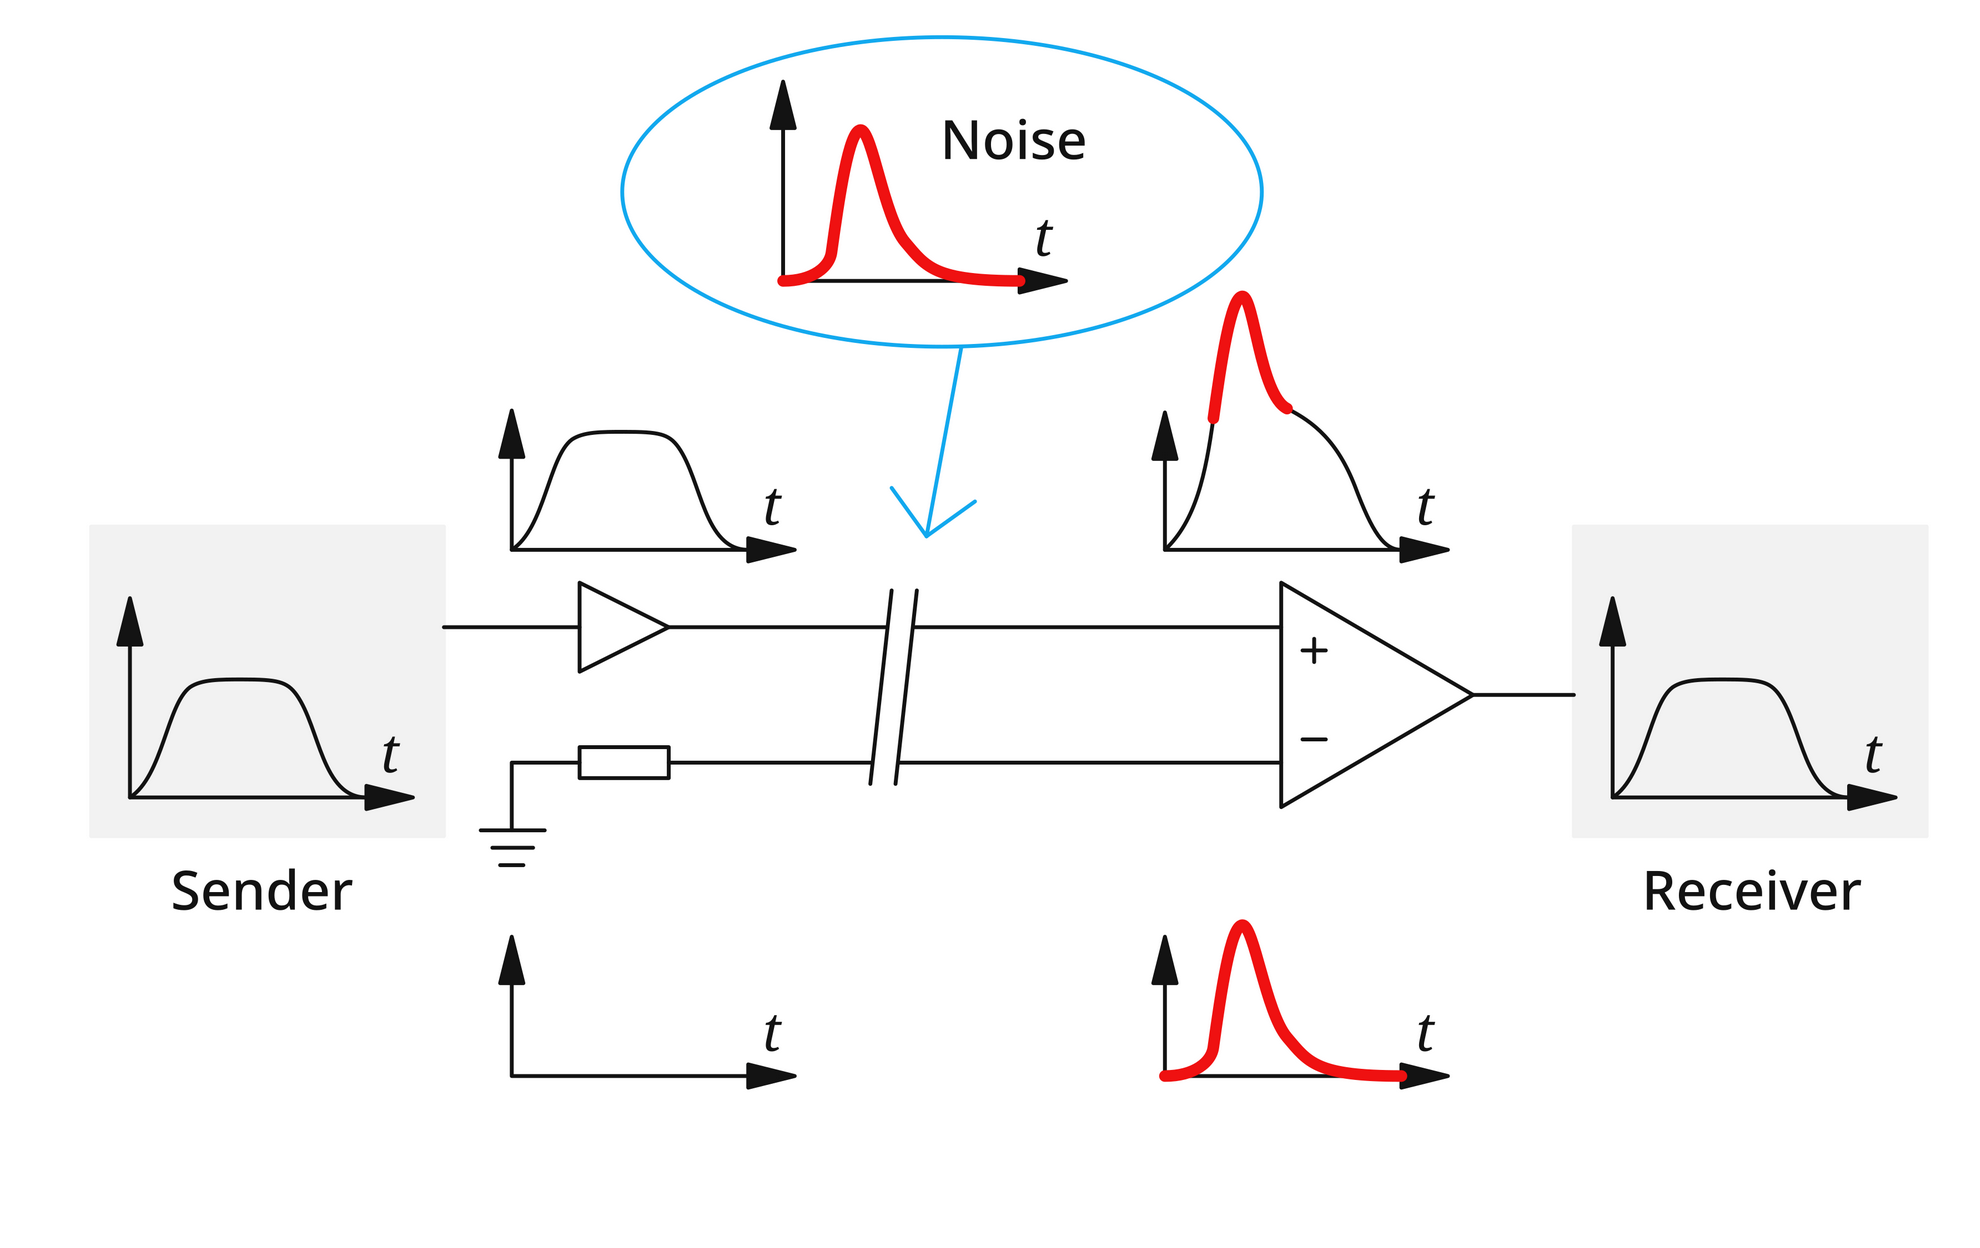
\includegraphics[scale=0.16]{../figures/common_mode_rejection.png}
\end{center}

\subsubsection{Amplificatori operazionali}
L'\textbf{amplificatore operazionale} è un caso particolare di amplificatore differenziale. Sostanzialmente rappresenta un amplificatore differenziale accoppiato in DC.

Nella pratica gli amplificatori operazionali sono costruiti su circuiti integrati, usando tecnologia a BJT o MOSFET, con un numero di transistor che va nell'ordine delle decine. 

Vengono chiamati amplificatori operazionali in quanto vengono impiegati per compiere \textit{operazioni} sui segnali, come moltiplicazione per costanti, integrare o derivare segnali, implementare tutta una serie di funzioni trascendenti, ecc...
Proprio per questo motivo sono stati i primi componenti utilizzati per realizzare i cosiddetti \textit{calcolatori analogici}.
Oggi questo impiego non è più così diffuso, ma gli amplificatori operazionali restano importanti per realizzare tutta quella classe di filtri denominati \textit{attivi}, cioè che implementano i filtri che modellizziamo in teoria di segnali attraverso funzioni matematiche.

Il simbolo dell'amplificatore operazionale è lo stesso che abbiamo visto per gli amplificatori differenziali:
\begin{center}
\begin{tikzpicture}[transform shape]
	% Paths, nodes and wires:
	\node[op amp, yscale=-1] at (0, -0){};
	\node[shape=rectangle, minimum width=0.465cm, minimum height=0.465cm] at (-1.44, 0.49){} node[anchor=center, align=center, text width=0.077cm, inner sep=6pt] at (-1.6, 0.49){$v_1$};
	\node[shape=rectangle, minimum width=0.465cm, minimum height=0.465cm] at (-1.44, -0.49){} node[anchor=center, align=center, text width=0.077cm, inner sep=6pt] at (-1.6, -0.49){$v_2$};
	\node[shape=rectangle, minimum width=0.465cm, minimum height=0.465cm] at (1.44, -0){} node[anchor=center, align=center, text width=0.077cm, inner sep=6pt] at (1.44, -0){$v_u$};
	\node[ground] at (-0.083, -0.539){};
	\node[vcc](N1) at (-0.083, 0.539){} node[anchor=south] at (N1.text){$v_{cc}$};
\end{tikzpicture}
\end{center}
dove abbiamo quindi:
\begin{itemize}
	\item Due ingressi, $v_1$ e $v_2$, che chiamiamo rispettivamente ingresso \textit{non invertente} ($+$) e ingresso \textit{invertente} ($-$);
	\item Un uscita $v_u$ da cui si ricava il segnale $K(v_1 - v-2)$, cioè la differenza fra ingresso non invertente e ingresso invertente, amplificata;
	\item Due morsetti che non disegneremo sempre, cioè l'alimentazione e il ground. In verità, esistono due modalità di impiego dell'amplificatore operazionale:
		\begin{itemize}
			\item Con un pin di alimentazione a ground, come in figura, e quindi l'altro ad un certo $\Delta V$ sopra questo;
			\item In alimentazione \textit{duale}, dove i due morsetti di alimentazione sono a $\pm V$, sopra e sotto il ground. Solitamente questi valori sono $\pm 5\, V$ o $\pm 12 \, V$.
		\end{itemize}
\end{itemize}

\subsubsection{Circuito equivalente dell'amplificatore operazionale}
Iniziamo a vedere come si modellizza dal punto di vista elettrico il comportamento dell'amplificatore operazionale:

\begin{center}
\begin{tikzpicture}[transform shape]
	% Paths, nodes and wires:
	\draw (-1, 1) to[american resistor, l={$R_{in}$}] (-1, -1);
	\draw (-1, 1) -- (-3, 1);
	\draw (-1, -1) |- (-3, -1);
	\node[shape=rectangle, minimum width=0.465cm, minimum height=0.465cm] at (-3.25, 1){} node[anchor=center, align=center, text width=0.077cm, inner sep=6pt] at (-3.5, 1){$v_1$};
	\node[shape=rectangle, minimum width=0.465cm, minimum height=0.465cm] at (-3.25, -1){} node[anchor=center, align=center, text width=0.077cm, inner sep=6pt] at (-3.5, -1){$v_2$};
	\draw (1, 1) to[american controlled voltage source, l={$A_{v_{OL}} v_{in}$}] (1, -1);
	\draw (1, 1) to[american resistor, l={$R_{out}$}] (3, 1);
	\draw (-3, -1) to[open, l={$v_{in}$}] (-3, 1);
	\draw (4.1, -1) to[open, l={$v_{out}$}] (4.1, 1);
	\draw (1, -1) -- (3, -1);
	\node[shape=rectangle, minimum width=0.465cm, minimum height=0.465cm] at (3.25, 1){} node[anchor=center, align=center, text width=0.077cm, inner sep=6pt] at (3.25, 1){$+$};
	\node[shape=rectangle, minimum width=0.465cm, minimum height=0.465cm] at (3.25, -1){} node[anchor=center, align=center, text width=0.077cm, inner sep=6pt] at (3.25, -1){$-$};
\end{tikzpicture}
\end{center}

Vediamo i componenti impiegati:
\begin{itemize}
	\item Come in qualsiasi circuito equivalente, abbiamo un'impedenza di ingresso $R_{in}$ e un'impedenza di uscita $R_{out}$. Per quanto abbiamo detto riguardo ai circuiti che implementano porte, vogliamo che nel caso ideale $R_{in}$ sia infinita, e $R_{out}$ nulla. Nella pratica riusciamo ad ottenere $1 - 3 \, M\Omega$ all'ingresso, e $10 - 30 \, \Omega$ all'uscita;
	\item Modellizziamo l'amplificazione attraverso un generatore di tensione pilotato in tensione da $v_{in}$, che sarà la nostra variabile di ingresso:
	$$
	v_{in} = v_1 - v_2 = v_d
	$$
	cioè il segnale in modo differenziale.
\end{itemize}

\par\smallskip

\noindent
\textbf{\textsf{Caratteristiche di merito}} \\
\noindent
Il guadagno dell'amplificatore operazionale $A_{V_{OL}} = A_d$ viene detto guadagno di \textit{Open Loop} (OL), cioè di catena aperta, in quanto molto spesso questi amplificatori vengono usati in catene reazionate. Vediamo che nell'amplificatore operazionale ideale il guadagno in catena aperta tende ad infinito. Nei casi reali, non raggiungiamo chiaramente l'infinito ma abbiamo comunque guadagni attorno a $10^5 - 10^6$.

Un'altra caratteristica fondamentale degli amplificatori operazionali è la \textit{banda}, in quanto ci dà una misura dei segnali a frequenza massima amplificabili, e della possibilità di stabilizzare l'amplificatore operazionale stesso in un circuito chiuso. Questo va nei modelli odierni sui $4-10 \, \mathrm{Hz}$.
Ancora più importante della banda ci risulta il \textit{prodotto guadagno-banda} (PGB), che idealmente vorremo portare all'infinito. Anche questo, essendo largamente dipendente dal guadagno, si aggira sui $10^5 - 10^6$. Il prodotto guadagno-banda è utile in quanto ci dà una migliore indicazione del guadagno che effettivamente rimane quando il componente viene inserito in un sistema retroazionato.
Infine, come abbiamo anticipato, caratteristica utile dell'amplificatore operazione è il CMRR, che sta intorno ai $90-120 \, \mathrm{dB}$.

\par\smallskip

Vediamo un ulteriore dettaglio, prendendo il circuito con alimentazione duale:
\begin{center}
\begin{tikzpicture}[transform shape]
	% Paths, nodes and wires:
	\node[op amp] at (0.083, -0.039){};
	\draw (0, 0.5) -| (0, 3) -- (4, 3) -- (4, 2);
	\draw (4, -2) -| (4, -3) |- (0, -3) -| (0, -0.578);
	\draw (4, 2) to[battery1, l={$v_{cc}$}] (4, -0);
	\draw (4, -0) to[battery1, l={$v_{ee}$}] (4, -2);
	\node[eground] at (5, -0){};
	\draw (4, -0) -- (5, -0);
	\node[shape=rectangle, minimum width=0.465cm, minimum height=0.465cm] at (-1.357, 0.451){} node[anchor=north west, align=left, text width=0.077cm, inner sep=6pt] at (-1.807, 0.701){$v_1$};
	\node[shape=rectangle, minimum width=0.465cm, minimum height=0.465cm] at (-1.357, -0.529){} node[anchor=north west, align=left, text width=0.077cm, inner sep=6pt] at (-1.807, -0.279){$v_2$};
	\node[shape=rectangle, minimum width=0.465cm, minimum height=0.465cm] at (1.523, -0.039){} node[anchor=north west, align=left, text width=0.077cm, inner sep=6pt] at (1.273, 0.211){$v_u$};
\end{tikzpicture}
\end{center}
In questo caso abbiamo preso una configuraizone dove si forniscono due \textit{rail} (in inglese rotaie) a $-v_{ee}$ e a $v_{cc}$ rispettivamente.

Se alimentiamo un amplificatore operazionale in maniera duale, cioè con 2 rotaie a $\pm V$, abbiamo che il valore di uscita è limitato al range $[-V, +V]$, cioè è impossibile oltrepassare i limiti dati dall'alimentazione. Abbiamo poi che in realtà nemmeno i limiti a $\pm V$ vengono raggiunti esattamente, e si ha uno scarto di alcuni volts attorno ad entrambe le rotaie a $\pm V$. Amplificatori operazionali con scarto minimo dalle rotaie vengono detti \textit{rail-to-rail} (dove lo scarto si aggira attorno al $0.1 \, \mathrm{V}$).

La caratteristica di uscita che otteniamo è quindi la seguente:
\begin{center}
	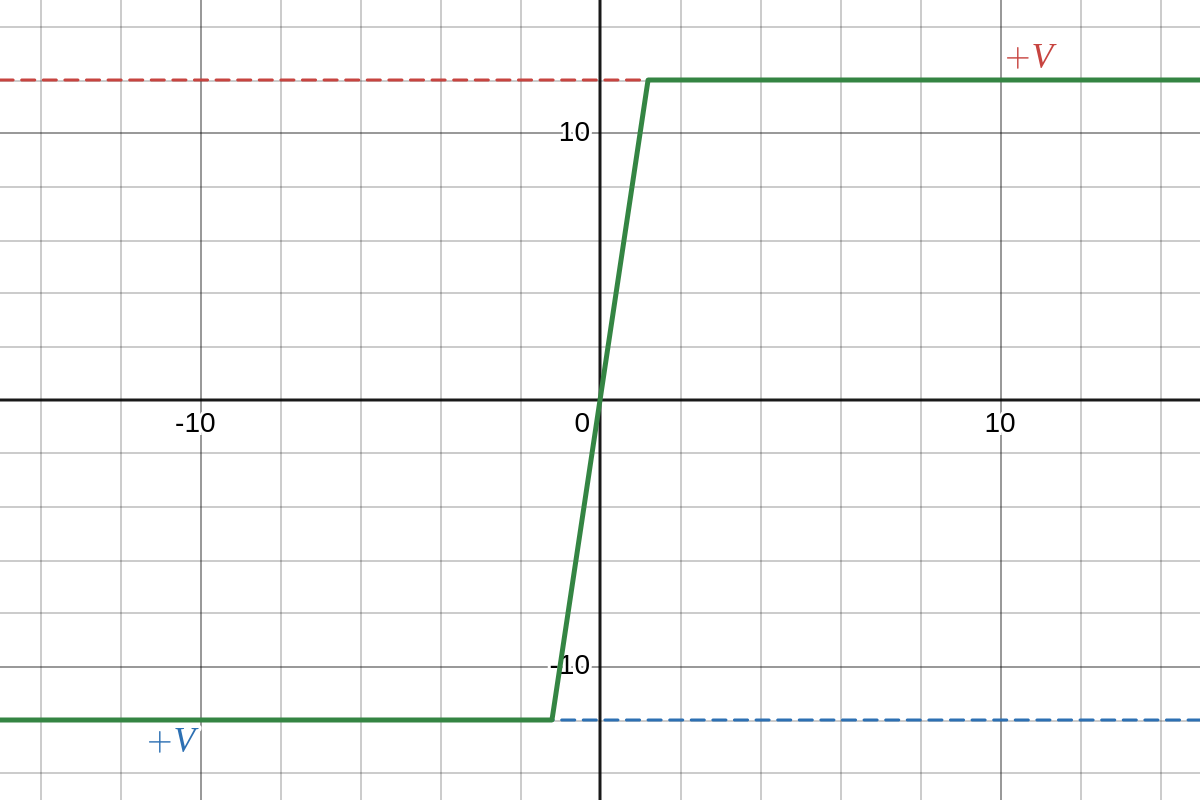
\includegraphics[scale=0.25]{../figures/op_amp_rail.png}
\end{center}
cioè la tensione in uscita segue linearmente quella in ingresso, amplificata per il guadagno di open loop $G_{OL}$, fino alle regioni di saturazione ottenute quando si incontrano le rotaie a $\pm V$:
$$
G_{OL} V_{in} = \pm V \implies V_{in} = \frac{V}{G_{OL}}
$$
Questo, unito al fatto che l'amplificatore operazionale ha solitamente un guadagno estremo, dà vita ad un componente che si trova quasi esclusivamente in saturazione (a minuscole variazioni di $v_{in}$ si passa da una regione di saturazione all'altra). Questo è giustificato dal fatto che quasi mai si usa l'amplificatore operazionale in catena aperta, ma lo si introduce in una catena chiusa col compito di stabilizzarne l'uscita. Contro di questo approccio è chiaramente che si ottiene un guadagno minore del guadagno di open loop $G_{OL}$.

In verità questo approccio è utile in quanto, assicurandoci che $G_{OL} >> 0$ sia generalmente enorme per qualsiasi amplificatore operazionale, ci assicuriamo che le caratteristiche di uscita saranno determinate dal circuito di reazione, e non dalle caratteristiche specifiche all'amplificatore operazionale stesso (che possono variare da modello a modello).

\subsubsection{Modello del cortocircuito virtuale}
Un modello di analisi per i circuiti ad amplificatore operazionale reazionato è quello a \textit{cortocircuito virtuale}.
Facciamo inanzitutto le seguenti ipotesi:
\begin{itemize}
	\item L'amplificatore operazionale è in zona lineare, per cui non siamo in saturazione;
	\item L'amplificatore operazionale è in un circuito chiuso, per cui il coefficiente di amplificazione in circuito chiuso $|\beta A| >> 1$;
\end{itemize}
Le conseguenze che otteniamo da qyeste ipotesi sono:
\begin{itemize}
	\item Dovrà essere che:$$V^+ \sim V^-$$ cioè possiamo assumere che queste siano in corto circuito (appunto, \textit{virtuale}), fra loro. Notiamo che questo cortocircuito è detto virtuale in quanto le tensioni a $V^*$ e $V^-$ sono sì uguali, ma la corrente che scorre fra questi è nulla (appunto perché sono a tensione uguale, ma imposta dall'esterno in retroazione anziché dalla conduzione di corrente);
	\item Come conseguenza di quanto detto sopra, dovrà essere anche che $$i^+ \sim i^- \sim 0$$
\end{itemize}

\subsection{Amplificatore non invertente}
Vediamo come si realizza un amplificatore \textit{non invertente} sfruttando un amplificatore operazionale.

\begin{center}
\begin{tikzpicture}[transform shape]
	% Paths, nodes and wires:
	\node[op amp] at (0, -0){};
	\draw (-1, 2) to[american resistor, l={$R_2$}] (1, 2);
	\draw (-1.75, 0.5) to[american resistor, l={$R_1$}] (-4, 0.5);
	\draw (-1.75, 0.5) -| (-1.19, 0.49);
	\draw (-1.19, 0.5) |- (-1, 2);
	\draw (1, 2) -| (1.19, -0);
	\draw (-1.19, -0.49) |- (-2, -0.5);
	\draw (-2, -0.5) to[american voltage source, l={$v_S$}] (-2, -2);
	\node[ground] at (-2, -2){};
	\node[ground] at (-4, 0.5){};
	\draw (1.19, -0) -- (2, -0);
	\node[shape=rectangle, minimum width=0.465cm, minimum height=0.465cm] at (2.25, -0){} node[anchor=center, align=center, text width=0.077cm, inner sep=6pt] at (2.25, -0){$v_u$};
\end{tikzpicture}
\end{center}

Ciò che facciamo quindi è, in breve:
\begin{enumerate}
	\item Prelevare un segnale $v_S$ ed inserirlo all'ingresso non invertente dell'OP amp;
	\item Partizionare il segnale $v_U$ di uscita fra le resistenze $R_2$ e $R_1$, e fornirlo in retroazione all'ingresso invertente dell'OP amp.
\end{enumerate}

Assumiamo che le ipotesi di cortocircuito virtuale siano soddisfatte e poniamo quindi le conseguenze:
$$
v^+ \approx v^-, \quad i^+ \approx i^- \approx 0
$$
cioè dovrà essere:
$$
v^+ = v_S = v^-, \quad i_1 = \frac{v_S}{R_1}, \quad i_2 = i_1
$$
dove la $i_1$ corre verso il ground a sinistra di $R_1$, e la corrente su $R_2$ (nella stessa direzione) può essere assunta come in cortocircuito sul polo invertente dell'OP amp (in quanto $i^- = 0$).

Possiamo quindi applicare il partitore di tensione:
$$
v_u = R_2 i_2 + R_1 i_1 = (R_2 + R_1) \frac{v_s}{R_1} = v_s \left( 1 + \frac{R_2}{R_1} \right) 
$$
Cioè si ottiene un guadagno:
$$
A = \frac{v_u}{v_s} = (1 + \frac{R_2}{R_1})
$$

Abbiamo quindi ottenuto un amplificatore con guadagno costante, dato da caratteristiche esterne al circuito (le 2 resistenze). Vediamo che il circuito è stabile in quanto le resistenze variano insieme sulla temperature e quindi rimangono pressoché costanti in rapporto, mentre le caratteristiche dell'OP amp (altamente variabili) non compaiono nemmeno nella formula del guadagno.

Se volessimo interrogarci sulla resistenza in uscita, da quanto detto riguardo alla teoria della reazione (scorsa lezione) abbiamo che questa è:
$$
R_{of} = \frac{R_{OPA}}{1 - \beta A} \approx 0
$$
dove $R_{OPA}$ è la resistenza di uscita dell'OP amp, abbiamo detto molto piccola.

La resistenza in ingresso sarà invece:
$$
R_i = \frac{v_s}{i_s} \rightarrow \infty
$$
in quanto la corrente $i^+$ all'ingresso va vicino a zero.

Abbiamo quindi raggiunto le caratteristiche di impedenza che consideriamo ideali: alta impedenza all'ingresso, minima impedenza all'uscita.

\subsubsection{Buffer}
Dalla configurazione ad amplificatore non invertente dell'amplificatore operazionale, impostato il guadagno a 1 (cioè la $R_2$ a 0) si ottiene un componente detto \textbf{buffer} o \textit{inseguitore di voltaggio}.
\begin{center}
\begin{tikzpicture}[transform shape]
	% Paths, nodes and wires:
	\node[op amp] at (0, -0){};
	\draw (-1.75, 0.5) to[american resistor, l={$R_1$}] (-4, 0.5);
	\draw (-1.75, 0.5) -| (-1.19, 0.49);
	\draw (-1.19, 0.5) |- (-1, 2);
	\draw (1, 2) -| (1.19, -0);
	\draw (-1.19, -0.49) |- (-2, -0.5);
	\draw (-2, -0.5) to[american voltage source, l={$v_S$}] (-2, -2);
	\node[ground] at (-2, -2){};
	\node[ground] at (-4, 0.5){};
	\draw (1.19, -0) -- (2, -0);
	\node[shape=rectangle, minimum width=0.465cm, minimum height=0.465cm] at (2.25, -0){} node[anchor=center, align=center, text width=0.077cm, inner sep=6pt] at (2.25, -0){$v_u$};
	\draw (-1, 2) -- (1, 2);
\end{tikzpicture}
\end{center}

Il buffer è quindi un amplificatore a guadagno unitario: risulta particolarmente utile quando si vuole separare un ingresso da un uscita, trasferendo comunque tensione da un capo all'altro.

Un buffer risulta particolarmente utile in situazioni dove si vuole governare un carico a bassa impedenza da una sorgente ad alta impedenza. Un carico a bassa impedenza tipico è ad esempio un altoparlante audio. Collegando l'uscita del circuito alimentatore direttamente al carico, si ottiene sostanzialmente un partitore di tensione fra l'impedenza dell'alimentatore $R_S$ e l'impedenza di carico $R_L$, per cui il segnale di uscita $V_u$ risulta:
$$
V_u = V_s \frac{R_L}{R_L + R_s} << 1
$$
e l'accoppiamento non è ideale.

Sfruttando un buffer, che governa direttamente il carico $R_L$, si impone a questo esattamente la tensione di ingresso $V_s$ senza ulteriori cadute. L'accoppiamento è quindi ideale, a patto che il buffer sia capace di fornire la corrente di cui il nostro carico ha bisogno.


\end{document}
